
%%%%%%%%%%%%%%%%%%%%%%%%%%%%%%%%%%%%%%%%%%%%%%%%%%%%%%%%%%%%%%%
% EDITORIAL SECTION
%
\documentclass{PSAIE}%

\usepackage{algorithm}
\usepackage{algpseudocode}

\sloppy
\begin{document}%
\PSAIEHeadFirst{10}{1}{1}{3}

% Please give a short title for the running head
\fancyhead[CO]{\PSAIEheader{Algorithmic extension of grapevine dataset for neural networks}}
\fancyhead[CE]{\PSAIEheader{Bal\'azs Bolyki, L\'aszl\'o \'Arvai and Dr. Szilvia \'Arvai-Homolya}}
\fancyfoot{}

\noindent\PSAIEtitle{Algorithmic extension of grapevine dataset for neural network}

\noindent\PSAIEauthor{Bal\'azs Bolyki}
{University of Miskolc, Hungary\\[0pt] Informatics Institute}
{bolyki@iit.uni-miskolc.hu}

\noindent\PSAIEauthor{L\'aszl\'o \'Arvai}
{University of Miskolc, Hungary\\[0pt] Informatics Institute}
{arvai.laszlo@iit.uni-miskolc.hu}

\noindent\PSAIEauthor{Dr. Szilvia \'Arvai-Homolya}
{University of Miskolc, Hungary\\[0pt] Mathematics Institute}
{mathszil@uni-miskolc.hu}

\noindent\PSAIEreceived{\today}

\noindent\PSAIEabstract{This paper is a template for those authors
      who wish to prepare their manuscript to be published in
      \emph{Production Systems and Information Engineering} by using the
      \emph{amsart} document class. You can reedit the text of this
      paper and the corresponding \emph{bib} file in order to obtain
      your manuscript.}

\noindent\PSAIEkey{dataset, grapevine}

\section{Introductions}
Robotization of grapevine pruning has become an area of interest in agriculture recently
\cite{botterill2017robot}, \cite{fernandes2021grapevine}, \cite{katyara2020reproducible}, since
tools for executing such a task are now available. Proper pruning requires expertise, and it is
a time consuming activity, resulting in expensive human workforce. Consequently, robotization is
a relevant alternative.

The pruning of grapevine means the removal of young, wooden canes of the plant, during the dormant session,
when the green parts are no longer present.
One of the subtasks of grapevine pruning is the reconstruction of the plant, based on images made by
one or multiple cameras, mounted on the robot. After plant reconstruction, the system can make decisions
as to where pruning has to be performed. Convolutional neural networks are available to do
object detection and localization on images \cite{glenn_jocher_2021_5563715}, \cite{matterport_maskrcnn_2017},
\cite{liu2016ssd}. However, such approaches require great amounts of training data. Creating a training
dataset of sufficient size and quality is laborous, and topic specific datasets are usually not available.
Also, existing neural networks do not provide their output in a proper format; at the time of writing,
there is no neural network with an output format, which could be directly utilized for pruning point
detection.

The desired output format of the plant reconstruction is a semantic graph, where graph nodes are parts
of the grapevine, and graph edges are connections between the parts. We aim to extend our existing
dataset towards such a graph format. In this paper, we achieve two goals. First, generating and
extending an existing, topic specific dataset, namely a bounding box based dataset created on grapevines.
Second, we use the current
bounding box data to retrieve more information on the grapevine structure, and convert the available
information to a more favorable format. In later sections we propose a methodology for generating a
new dataset algorithmicly, based on the original dataset, using area specific knowledge on the
grapevine, while requiring as little human intervention as possible. We also demonstrate how well a
neural network performs on purely machine generated data.

\section{Survey} \label{sec_survey}
Multiple papers address the issue of automated grapevine pruning. There are descriptions of complete,
functioning robot systems \cite{botterill2017robot}, and subtask descriptions of smaller scope
\cite{goesmannai}, \cite{fernandes2021grapevine}, \cite{katyara2020reproducible}.

When robotizing grapevine pruning, plant anatomy detection needs to be addressed. The thesis
\cite{white_background_grape} uses a purely algorithmic approach, analysing the grapevine plant
in front of a white background. However, taking images on grapevine plantation with white background
is problematic -- the author of the thesis took the pictures indoor. Background removal could also be
done by using the robot itself to block vision. In \cite{botterill2017robot} the background is not
visible, because the robot moves over the row grapevines and covers the plants in its U shaped form;
however, such a construct is very large and hard to transport.

In \cite{you2021semantics} robotic pruning of cherry trees is based on information retrieved by a
semantic segmentation neural network, then converted to skeleton format. Other
agricultural works use semantic or instance segmentation -- the paper \cite{chen2021semantic} uses semantic
segmentation for detecting apple trees, while \cite{santos2020grape} uses instance segmentation to count
grapes.

Authors addressing pruning point determination work on data in graph format \cite{goesmannai}, which is best
resembled by the skeleton format. Though skeleton format is desired for the output of the detector system,
we found no papers describing such neural networks, which directly returns skeletons for grapevine.
It is more viable to retrieve skeleton data, based on \cite{you2021semantics} semantic segmentation networks.

\section{Task description} \label{sec_task_description}
In this paper we describe a continuation of the thesis \cite{bolyki_2021}, where a bounding box based training
dataset was created, and the YOLO (You Only Look Once) neural network was trained
\cite{glenn_jocher_2021_5563715}.
A bounding box based dataset can be created relatively quickly, but it does not fit the task of pruning
point detection well. However, results retrieved in bounding box format are reliable, and -- provided task
specific information -- could be appropriately converted and used to attain more information, such as
the relationships between the detected grapevine parts.

We have access to a large set of images taken on a grapevine plantation, with the usage of a white screen
for background, and we also have images without any white background at all. One of the images with
white background is presented on Figure \ref{fig_grapevine_image}.
We make use of the original \cite{bolyki_2021} trained neural network to create a more desired
format for representing grapevine detections. The original format uses bounding boxes for
representation, and detects four different classes of grapevine parts:
\begin{enumerate}
      \item \textbf{trunk},
      \item \textbf{cordon} -- the old, thick part of the grapevine, running on the trellis wires horizontally,
      \item \textbf{arm} -- old, usually vertical branches, providing a base for canes to grow,
      \item \textbf{node} -- young proturbances on the canes containing multiple buds from which new parts
            can grow.
\end{enumerate}

\begin{figure}[h]
      \centering
      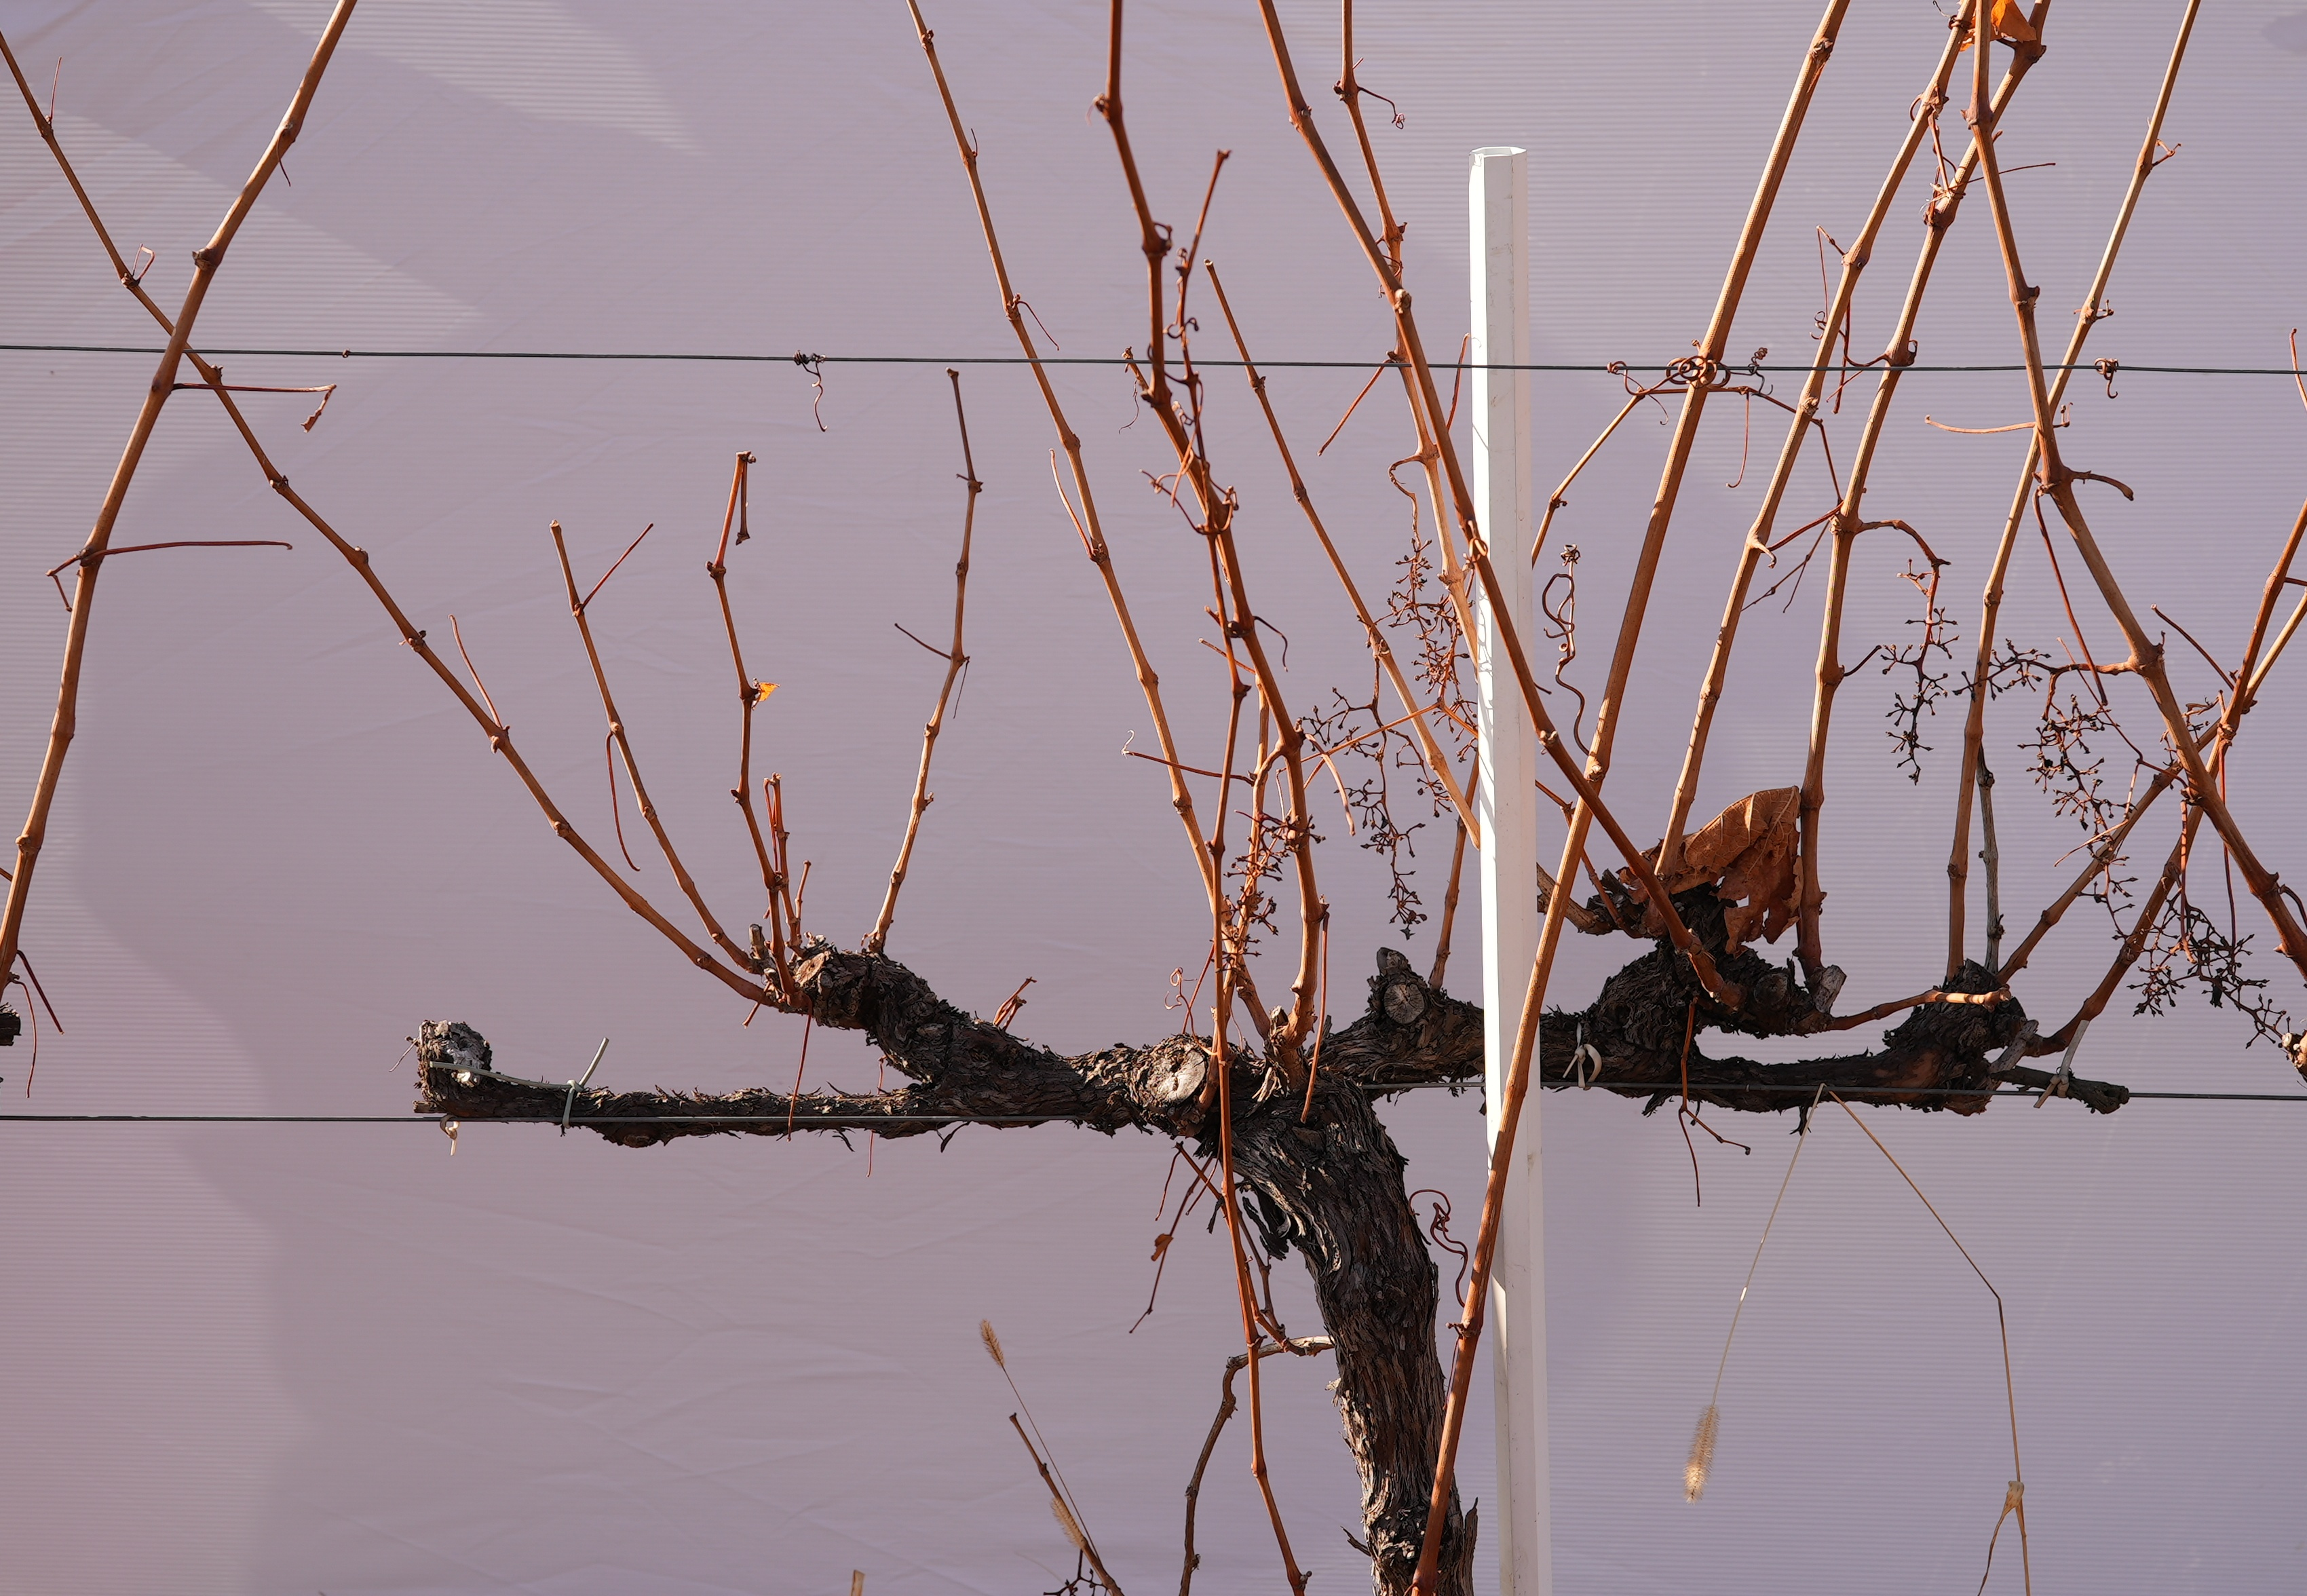
\includegraphics[scale=0.08]{images/grapevine_image.jpg}
      \caption{Grapevine image}
      \label{fig_grapevine_image}
\end{figure}

Parts of the grapevine are represented on Figure \ref{fig_grapevine_structure}. It is best to further clarify
the meaning of node, bud, cane, internodium. Canes are young -- one year old -- wooden branches of the
grapevine, which consist of nodes -- spherical proturbances --, and internodiums -- straight wooden organs
connecting the nodes. Buds can yield shoots (canes before lignification -- turning to wood), leaves, tendrils,
flowers, and they grow on nodes. To determine pruning points we need to know where the canes are, where their
nodes are, where they start -- do they grow from arms, cordons or the trunk --, and how many canes grows from
a single arm. We practically have to build a graph of nodes, internodiums, arms, cordons, etc. to represent
their relationships.

\begin{figure}[h]
      \centering
      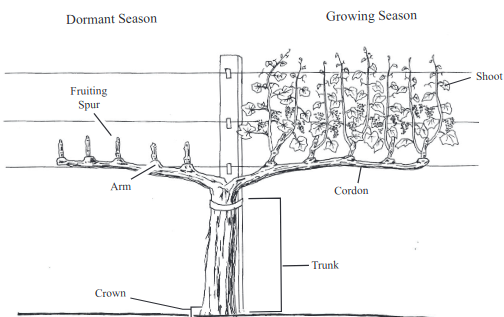
\includegraphics[scale=0.7]{images/grapevine_structure.png}
      \caption{Grapevine structure \cite{hellman2003grapevine}}
      \label{fig_grapevine_structure}
\end{figure}

By extending the available dataset we mean multiple things.
\begin{enumerate}
      \item The available dataset could be extended purely in quantity. Since the accuracy of a neural network
            depends greatly on both the size and quality of the dataset, this extension is valuable.
            By running the detection script of the YOLO neural network on a large set of new images,
            we attain great amounts of new training images. However, these almost always require
            manual correction.
      \item We extend the dataset by adding a new class to the original four, which could be named \textit{cane}
            or \textit{internodium} depending on the extension format. This requires algorithmic detection of
            objects of the new class.
      \item We extend the dataset by adding new logical formats, meaning we use the original bounding box
            detections to create both skeleton and semantic segmentation datasets.
\end{enumerate}

\section{Internodium detection} \label{sec_internodium_detection}
Internodium detection is performed on pictures taken on grapevine plantations. On these images, white
background was used -- allowing us more operations on the grapevine, such as segmentation, background
switching and building of canes or detecting internodiums.

Detection of internodiums is performed by building canes, based on the nodes found by the pretrained YOLO
neural network \cite{bolyki_2021}, \cite{glenn_jocher_2021_5563715}. The pretrained YOLO network is used
to retrieve the bounding boxes representing the trunks, cordons, arms and nodes on the image. Figure
\ref{fig_grapevine_YOLO}. represents one of the outputs of the YOLO network.

\begin{figure}[h]
      \centering
      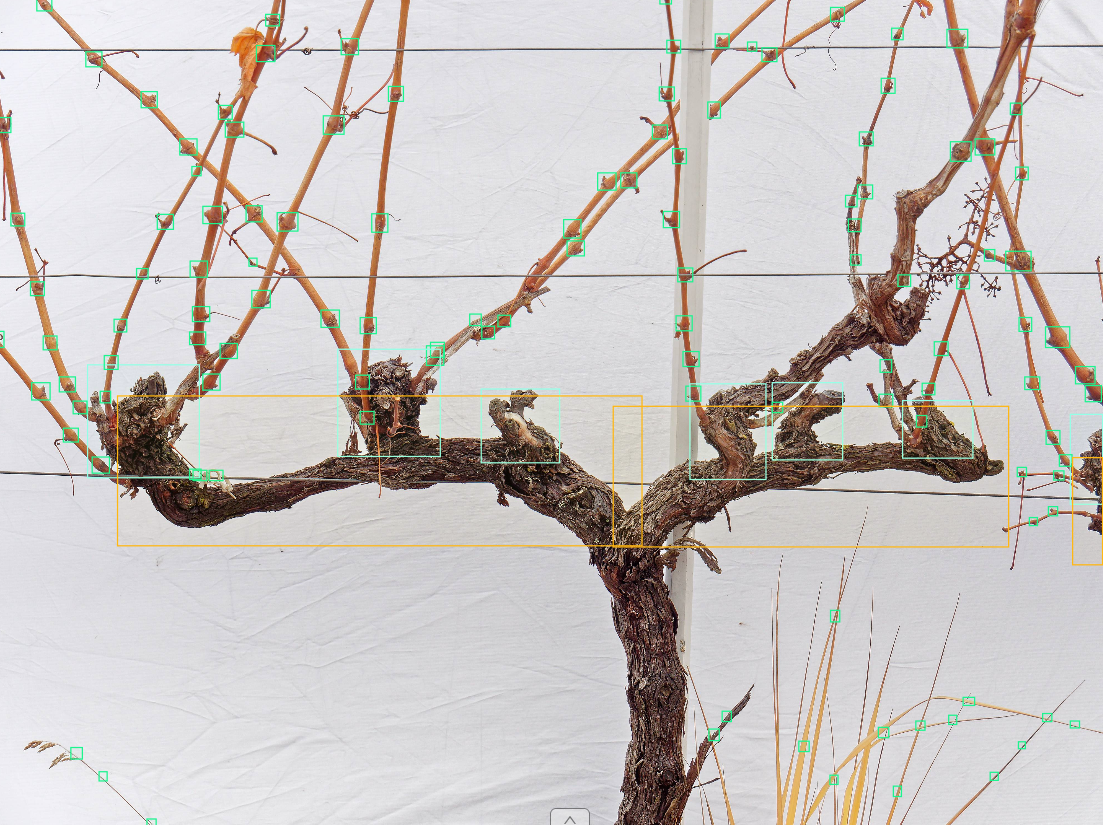
\includegraphics[scale=0.28]{images/grapevine_yolo.png}
      \caption{Grapevine detections \cite{hellman2003grapevine}}
      \label{fig_grapevine_YOLO}
\end{figure}

After the starting bounding box detections are retrieved, the steps of internodium detection are the following:

\begin{enumerate}
      \item Create color masks for the young parts of the grapevine: internodiums, nodes.
      \item Build the cane starting from a specific node.
      \item Store the connections between the nodes of the cane, thereby storing the internodiums.
\end{enumerate}

In this section we describe these steps in more detail.

\subsection{Create color masks} \label{sec_create_color_masks}
Since the pictures taken on the grapevine plantation have white backgrounds, separating the grapevine
from the background by color is perfectly viable. Also, it is possible to separate the older and the
younger parts of the grapevine from each other. In order to do so, we make use of the OpenCV
(Open Source Computer Vision)
library \cite{opencv_library}. The library contains a large set of optimized image processing and computer
vision algorithms. We use it for loading images, converting colors, executing morphological operations.

To separate the younger and older parts of the image from the background, we first convert the images
to HSV color space (Hue-Saturation-Value) from OpenCV's default (BGR -- Blue-Green-Red). Based on the
HSV value of pixels we generate binary masks for both young and old parts of the cane, where the size
of the mask matches the image, and each field of the mask is set to true -- represented by the number 255,
since OpenCV does not support actual binary masks -- if its color is within a specified range.

The ranges specified for the young and the old parts are the following:

\begin{itemize}
      \item \textbf{Young part (cane)}: $hs > 60 \wedge hv > 70$
      \item \textbf{Old part (arm, cordon, trunk)}: $hs > 10 \wedge hv <= 70$
\end{itemize}

\subsection{Build cane} \label{sec_build_cane}
In order to find connections between the nodes, we attempt to build canes on the image. To do this,
we take the following steps:
\begin{enumerate}
      \item Sort nodes in top-down order. Start iteration from the upmost node.
      \item If the next node is not yet connected to any other node, then name it $startNode$, and continue
            with next step, otherwise repeat this step.
      \item Find a $buildTries$ number of nodes that can be best connected to $startNode$ based on Algoritm
            \ref{alg_trace_line}., which returns a probability. Name these $bestNodes$.
      \item For each best point try to build a cane with Algorithm \ref{alg_build_cane}.
            Accept and store the longest cane and discard the rest.
      \item If all nodes that are not part of a cane were tried as $startNode$, then exit. Otherwise go to step
            2.
\end{enumerate}

Algorithm \ref{alg_trace_line}. returns an estimated probability to whether two nodes are connected or not.
Algorithm \ref{alg_build_cane}. attempts to build a cane, and returns the cane when it is finished; if the
algorithm cannot build a cane, then it returns the original two nodes, which were passed to it as arguments
-- these compose the cane.

The can\_wander\_to\_cane part of Algorithm \ref{alg_trace_line} is a utility function, which is given
a $p$ point and a line. The function attempts to "wander off" the line, and takes a point $steps$ distance from the
line in both positive and negative directions: $\vec{ps}^-$, $\vec{ps}^+$. If the line is slopey --
$\vec{v} = \vec{p2} - \vec{p1}; \vec{v} = (vx, vy); |vx| < |vy|$ -- then we take the steps horizontally,
$\vec{ps}^- \gets (vx - steps, vy), \vec{ps}^+ \gets (vx + steps, vy)$, otherwise we take them vertically
$\vec{ps}^- \gets (vx, vy - steps), \vec{ps}^+ \gets (vx, vy + steps)$. The can\_wander\_to\_cane function
returns true if either the pixel on $\vec{ps}^-$ or on $\vec{ps}^+$ has the color of the cane.

\begin{algorithm}
      \caption{Trace along line}
      \label{alg_trace_line}
      \begin{algorithmic}
            \Function{traceAlongLine}{$\vec{p1}$, $\vec{p2}$, $plimit$}
            \Comment Inputs are the endpoints of the line and a limit: $\vec{p1}$, $\vec{p2}$, $plimit$
            \State $points \gets$ points along the line
            \State $\vec{p}\gets \vec{p1}$
            \State $len \gets$ length of line
            \State $caneCount \gets 0$
            \State $noncaneCount \gets 0$
            \State $limit = len * plimit$; \Comment{$plimit$ percent of line is allowed to be non-cane}
            \While{$\vec{p} \neq vec{p2}$ \textbf{and} $noncane \leq limit$}
            \If{$\vec{p}$ is potential cane by color \textbf{or} can\_wander\_to\_cane}
            \State $cane = cane + 1$
            \Else
            \State $noncane = noncane + 1$
            \EndIf
            \State $\vec{p} \gets$ next point on line
            \EndWhile
            \State $prob = cane / len$
            \State \textbf{return} $\gets prob$
            \EndFunction
      \end{algorithmic}
\end{algorithm}

The viability checks in Algorithm \ref{alg_build_cane}. are based on preconfigured values.

\begin{itemize}
      \item The angle of a node triplet is considered viable if the cosine of the angle is below $-0.8$,
            which is a preconfigured angle cosine maximum.
      \item The distance $\delta = d(lastNode, newNode)$ of two nodes is viable if the difference between
            $\delta$ and $\delta' = d(prevNode, lastNode)$ is no greater then $\delta' * 0.7$, which is a
            preconfigured length difference limit.
      \item $traceAlongLine(lastNode, bestNextNode, plimit)$ is viable if it reaches a preconfigured
            probability minimum, which we have set to 0.6.
\end{itemize}

\begin{algorithm}
      \caption{Build cane}
      \label{alg_build_cane}
      \begin{algorithmic}
            \Function{buildCane}{$n1$, $n2$} \Comment Inputs are the first two points of the cane
            \State $plimit$ is preconfigured
            \State $cane \gets n1, n2$, where $cane$ is a list of nodes
            \State $prevNode \gets n1$
            \State $lastNode \gets n2$
            \State $couldGrow \gets true$
            \While{$couldGrow$}
            \State $nodes \gets$ nodes within a distance from $lastNode$.
            \State $couldGrow \gets false$
            \State $bestNextNode \gets NULL$
            \For{$nextNode$ in $nodes$}
            \If{$(prevNode, lastNode, nextNode)$ angle is viable\\
                  \textbf{and} distance of $(lastNode, nextNode)$ is viable\\
                  \textbf{and} $traceAlongLine(lastNode, bestNextNode, plimit)$ is viable}
            \State $p = traceAlongLine(lastNode, bestNextNode, plimit)$
            \State $p' = traceAlongLine(lastNode, nextNode, plimit)$
            \State if $p < p'$ then $bestNextNode \gets nextNode$
            \EndIf
            \EndFor
            \If{$bestNextNode != NULL$}
            \State $couldGrow = true$
            \State $cane \gets bestNextNode$ \Comment add new node to cane
            \State $prevNode \gets lastNode$
            \State $lastNode \gets bestNextNode$
            \EndIf
            \EndWhile
            \State \textbf{return} $\gets cane$
            \EndFunction
      \end{algorithmic}
\end{algorithm}

\subsection{Conclusion} \label{sec_build_cane_conclusion}
The result of the algorithm is an estimation of the canes. One estimation is represented in Figure
\ref{fig_grapevine_connections}.

\begin{figure}[h]
      \centering
      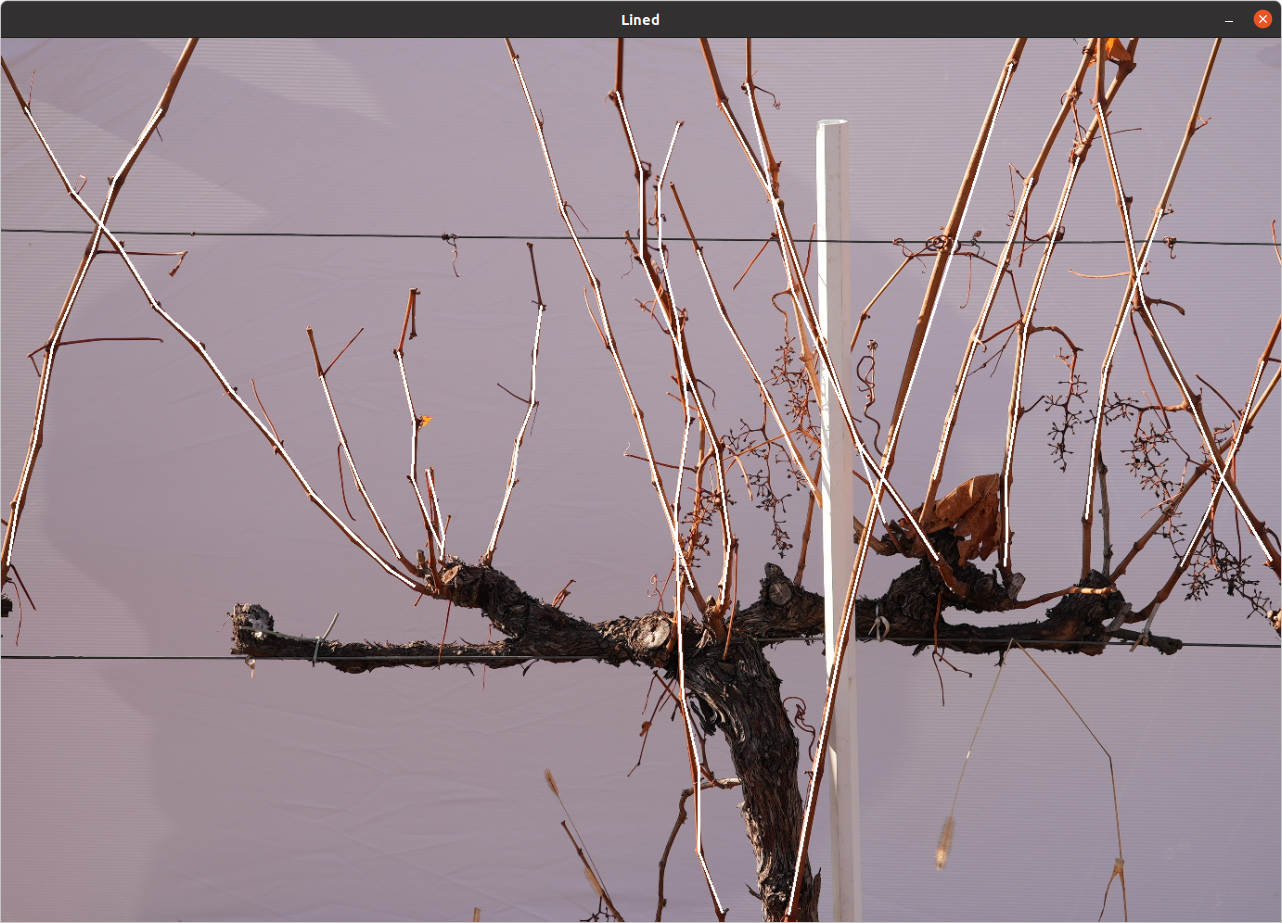
\includegraphics[scale=0.28]{images/grapevine_connections.png}
      \caption{Grapevine connections}
      \label{fig_grapevine_connections}
\end{figure}

The algorithm has two main deficiencies:
\begin{enumerate}
      \item When canes on the picture cross over each other, then it cannot reliably tell which cane is which, since
            we do not have 3D data to support such decisions.
      \item White background is required for the algorithm to work.
\end{enumerate}

We note that the above described algorithm starts from the top left node and goes left to right, top to bottom.
This usually results that the canes are built from their end towards their beginning. This is due to one of the
deficiencies of the algorithm: its inability to handle overlapping canes. On the top of the canes, there are
less overlaps, and there are less first best connections to try; consequently, there are less attempts required to
build a cane.

We cannot use the output of this algorithm to make reliable pruning decisions, but we can use it to generate
train data. The exporting of cane data is discussed in the next section.

\section{Exporting data} \label{sec_exporting_data}
Once we have retrieved cane information from the image, we can export it in other format, so we can use it for
training neural networks. We implemented and tested two export formats:

\begin{enumerate}
      \item bounding box format,
      \item polyline format.
\end{enumerate}

\subsection{Bounding box format} \label{sec_export_bounding_box_format}
To export canes as bounding boxes, we need to break the cane down into nodes and internodiums. Such a
breakdown is shown in Figure \ref{fig_internodium_boxes}.

\begin{figure}[h]
      \centering
      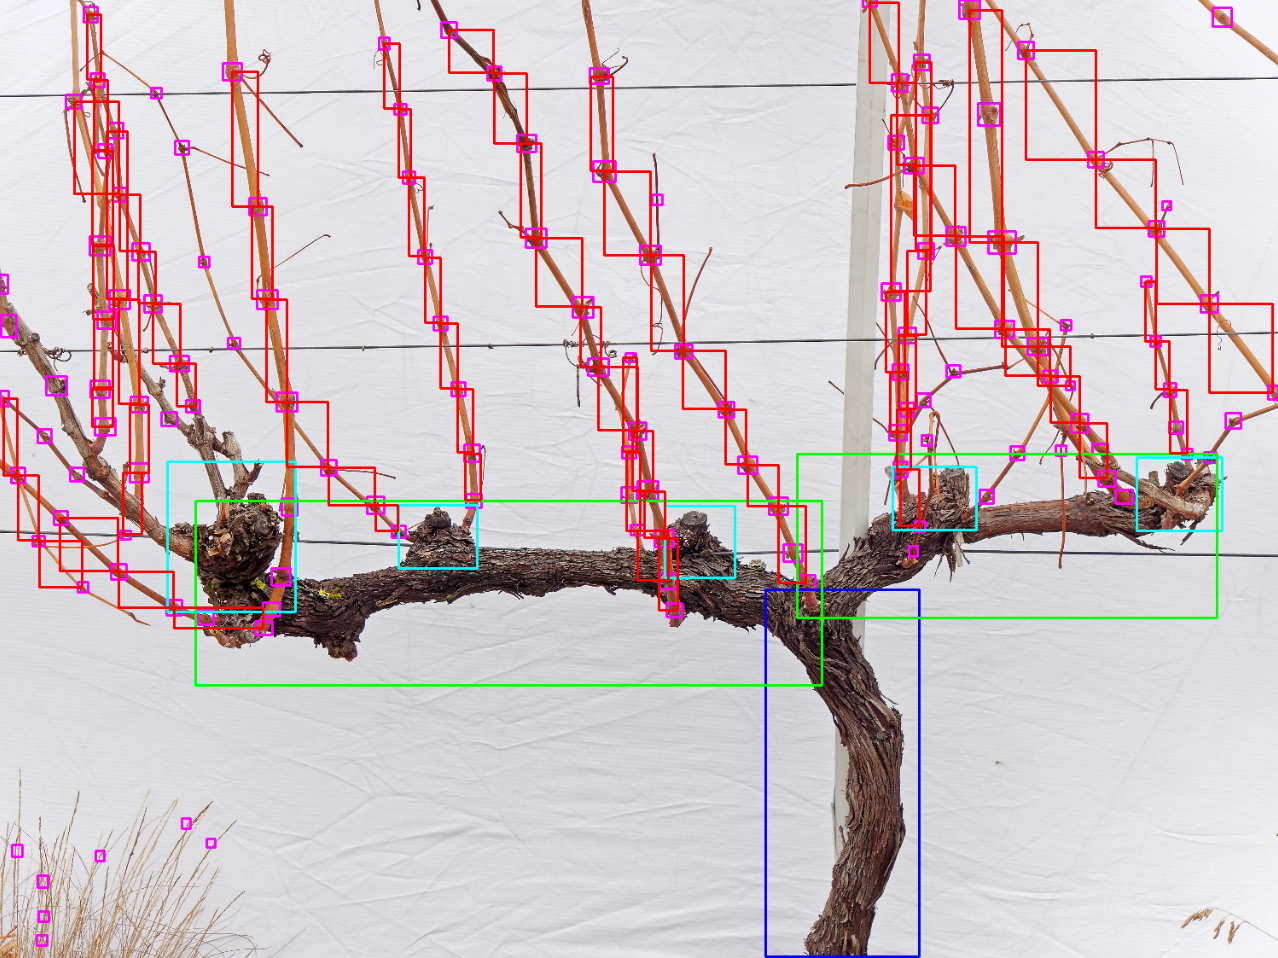
\includegraphics[scale=0.28]{images/internodium_boxes.png}
      \caption{Canes as nodes and internodiums}
      \label{fig_internodium_boxes}
\end{figure}

To store
bounding boxes for nodes and internodiums we use the YOLO annotation format. The advantage of this format
is that it could be given to the YOLO neural network for training and validation. The YOLO format takes image
and text file pairs, where the image file is the annotated picture, and the text file contains the annotation.
The annotation in the text file consists of one line per bounding box. One line in the text file looks like
this:

\textit{class x y w h}

Here, \textit{class} is an integer number representing the class of the detected object, \textit{x} and
\textit{y} are floating point numbers in the range of 0-1 marking the \textit{center} coordinates of the
bounding box, and \textit{w} and \textit{h} are also floating point numbers between 0 and 1 holding the
value of the width and height of the bounding box.

We should note that the YOLO format cannot store connection data directly; we can only assume the existence
of connections based on the positions of bounding boxes. Consequently, data loss would possibly occur
when using stored data.

In Section \ref{sec_use_of_generated_data}. we show usage of generated YOLO data.

\subsection{Polyline format} \label{sec_export_polyline_format}
We can use polyline format for testing and further annotation. A cane of the grapevine cannot effectively
be represented as a single bounding box, but could be given as a polyline. In this case, we represent the cane
as a sequence of point coordinates, where a point represents the center of a node, and each consecutive
node has a connecting internodium between them.

The export format of the polylines is the CVAT -- Computer Vision Annotation Tool -- output format for
images \cite{boris_sekachev_2020_4009388}, which uses XML based annotation. We add a polyline annotation
to an image by creating an XML tag for the polyline -- inside the image tag --, then list the coordinates
as an attribute to the polyline. CVAT is a tool for annotating images, so we can further improve the
annotation manually, then export it to a more commonly used format -- CVAT supports YOLO, Pascal VOC, COCO,
TFRecord, and a lot of other formats.

The advantage of this format is that the connection data is stored directly -- no loss occurs this way.
The disadvantage is that we have no knowledge of a polyline detection neural network that could make use of
this data.

\section{Use of generated data} \label{sec_use_of_generated_data}
We used the generated bounding box data -- described in Section \ref{sec_export_bounding_box_format}. --
to train a new YOLO neural network. This neural network was able to detect internodiums as well as the
previously annotated nodes, arms, cordons and trunks. An example run of the newly trained neural network
is shown in Figure \ref{fig_generated_data_train}. The given output was achieved with purely generated
data.

\begin{figure}[h]
      \centering
      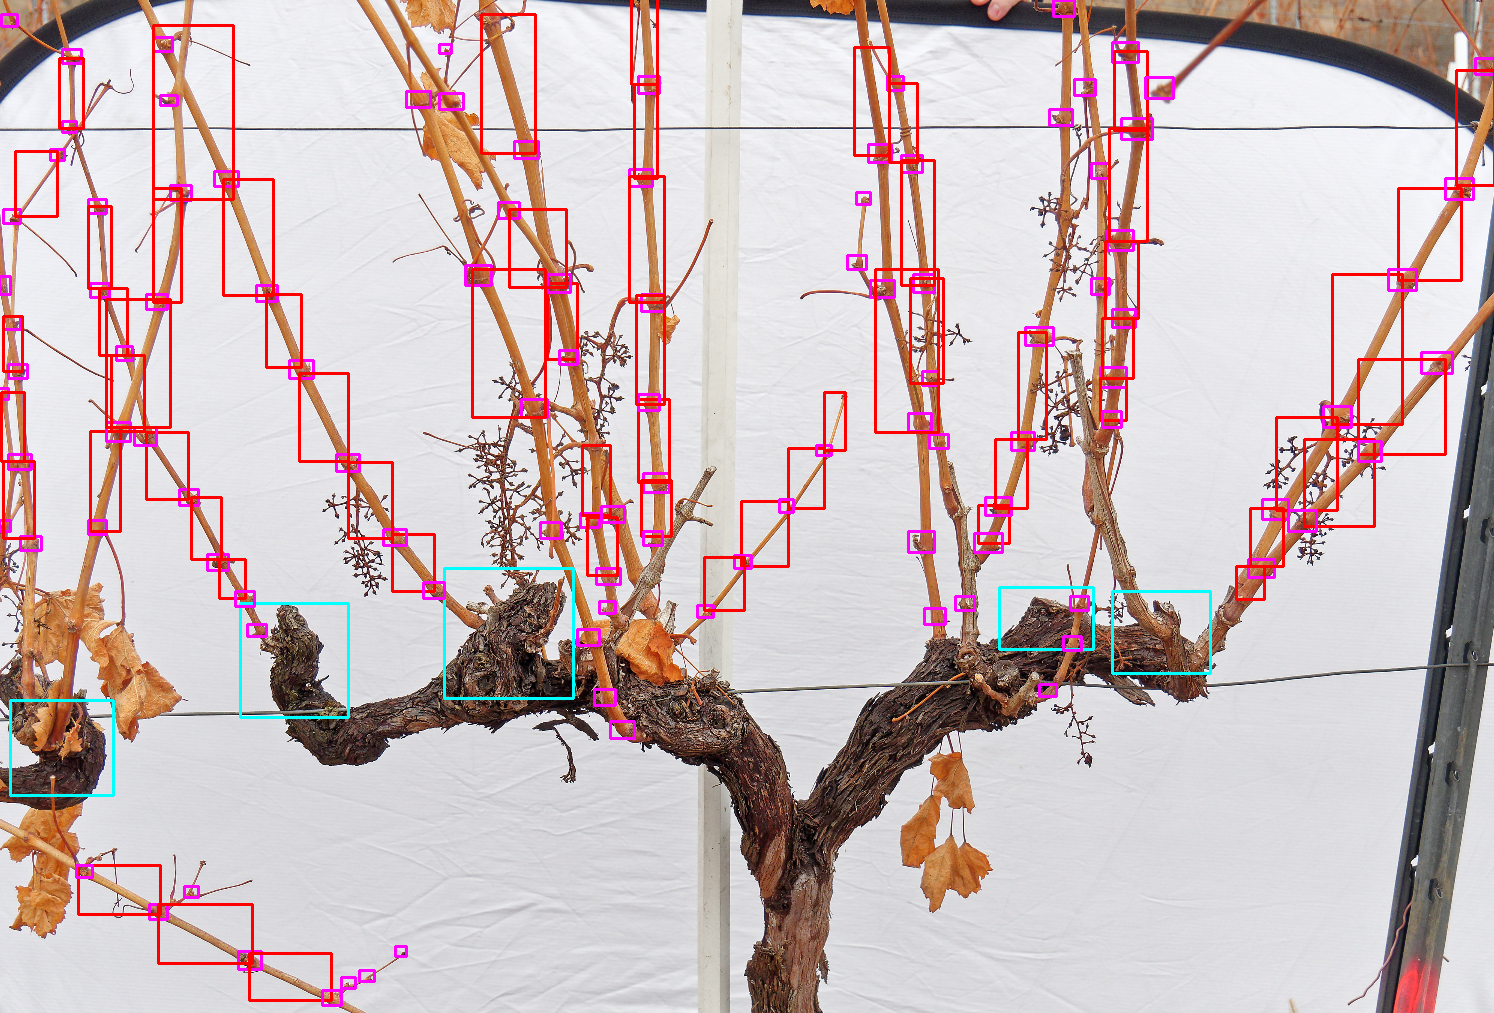
\includegraphics[scale=0.23]{images/generated_train_data.png}
      \caption{Neural network trained on generated data}
      \label{fig_generated_data_train}
\end{figure}

The disadvantage of using purely generated data is the unreliability of accuracy measurements; since the
validation data is also generated, Mean Average Precision, Precision, Recall have little meaning. In order
to reliably use and test such a neural network, manual correction are necessary. However, the amount of time
required for manual corrections is greatly reduced by generating a base annotation; hundreds of annotations
like the one visible on Figure \ref{fig_generated_data_train}. can now be generated in the matter of seconds,
greatly extending the available dataset.

Another advantage of extending the dataset with internodiums is that the reconstruction of canes
would no longer have to rely on the white background. For example, the output visible on Figure
\ref{fig_internodium_connections}. was generated without reliance on white background. The algorithm
connected all nodes which were connected by an internodium box -- where \textit{connected} means that the
internodium box had two diagonally opposite corners inside two different node boxes.

\begin{figure}[h]
      \centering
      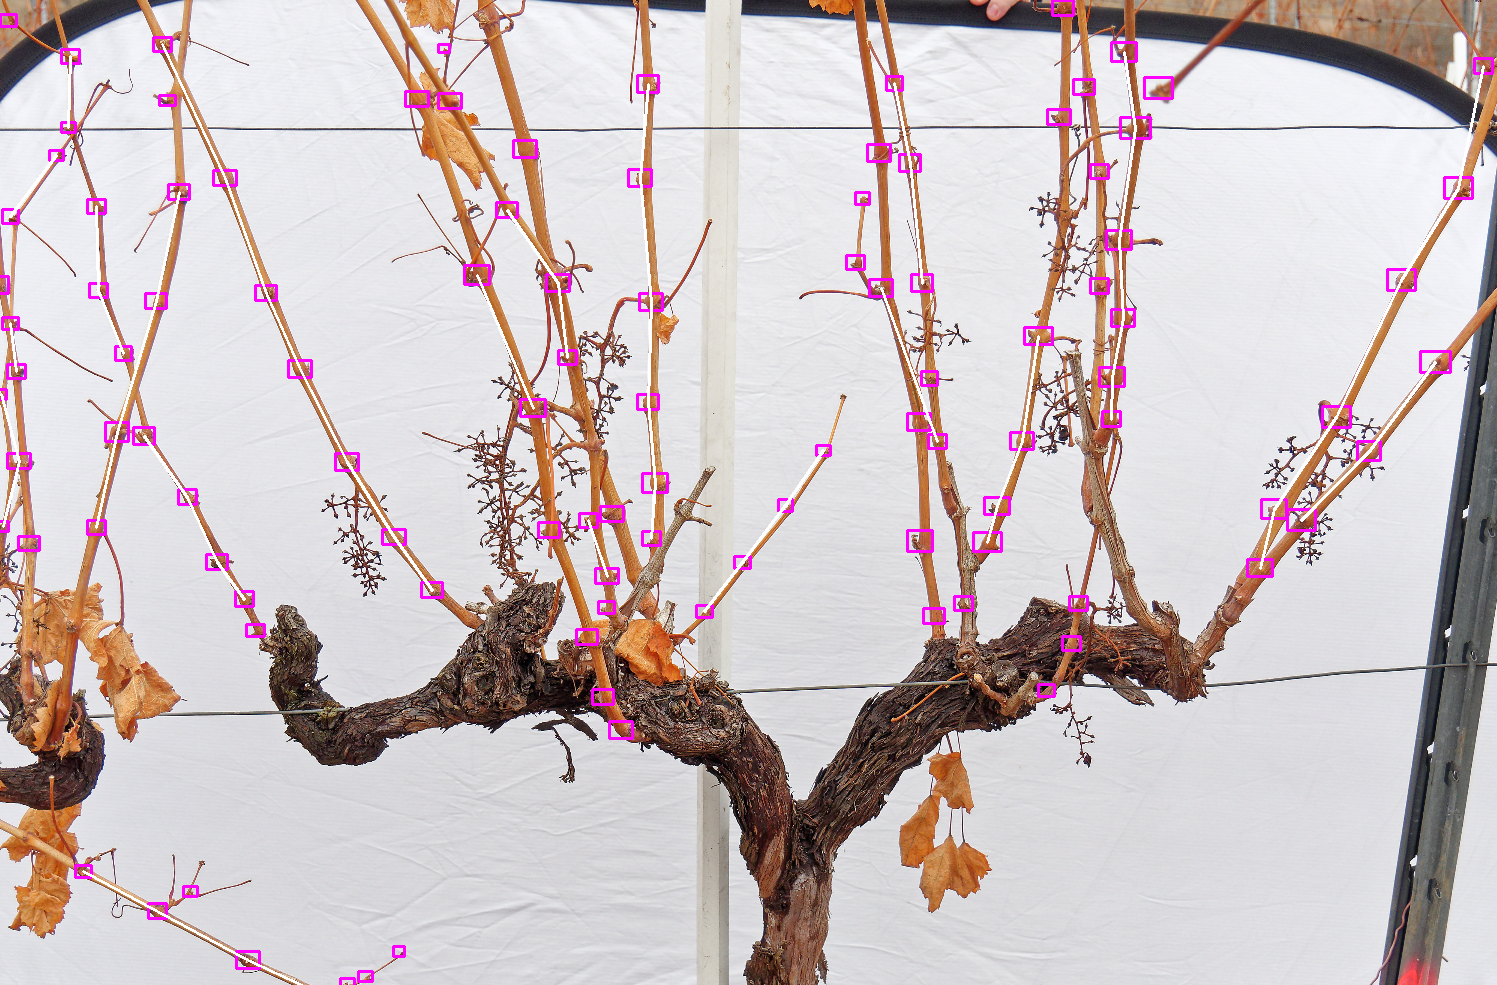
\includegraphics[scale=0.23]{images/internodium_connections.png}
      \caption{Cane reconstruction based on internodium boxes}
      \label{fig_internodium_connections}
\end{figure}

The reliability of the algorithm is now dependent on the accuracy of the YOLO neural network -- which in
turn is dependent on the size and versatility of the dataset.

\section{Conclusion} \label{sec_conclusion}
In this paper, we showed a methodology to extend a currently available dataset to contain more images and
more classes of objects. Namely, the bounding box based dataset on grapevine images formerly contained
four classes of objects -- nodes, arms, cordons and trunks --, and now the class of internodium is
algorithmicly added to them. In case we export the dataset not as bounding boxes, but as polylines,
the detected canes can be accurately represented.

We used the algorithical extension of the dataset to teach a new neural network, which can now detect
internodiums too. Internodium detection can relieve us from the currently necessary white background,
making the photographing and reconstruction of grapevines much less demanding. Algorithmic dataset
extension reduces the human working hours required to create a large dataset.

\bibliographystyle{PSAIEbib}
\bibliography{citations}

\end{document}